  
\documentclass[12pt,a4paper,fleqn]{tufte-handout} 
\usepackage{graphicx} 
\usepackage{morefloats} 
\usepackage{amsmath} 
\usepackage{amssymb} 
\usepackage{rotating} 
% mcode options for matlab code insertion bw (for printing), numbered (line numbers), framed (frame around code blocks), useliterate (convert Matlab expressions to Latex ones), autolinebreaks (automatic code wraping, use it with caution 
\usepackage[literate]{mcode} 
\graphicspath{{figures/}{tex/}{../figures/}{../../}{../}}  
\title{classifyData} 
\author{ Mathieu Lagrange } 
  
\begin{document} 
  
\maketitle 
  
% Please use this file to document your experiment 
% You can compile the report by setting the option 'report' as detailed in your expLanes configuration file. 
  
\section{Introduction}

This report documents the third demonstration of the use of the expLanes framework to conduct a computational experiment. The project classifyData is about the comparison of two classifiers over synthetic data.

\section{Design}

\begin{marginfigure}
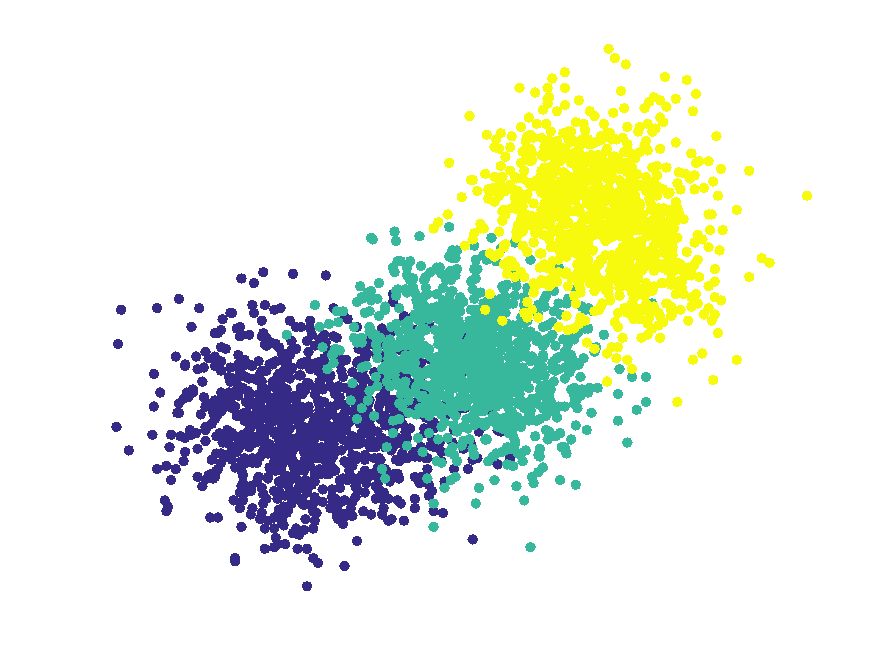
\includegraphics[width=\textwidth]{figures/scatter1}
\caption{The training dataset.}
\label{train}
\end{marginfigure}

\begin{marginfigure}
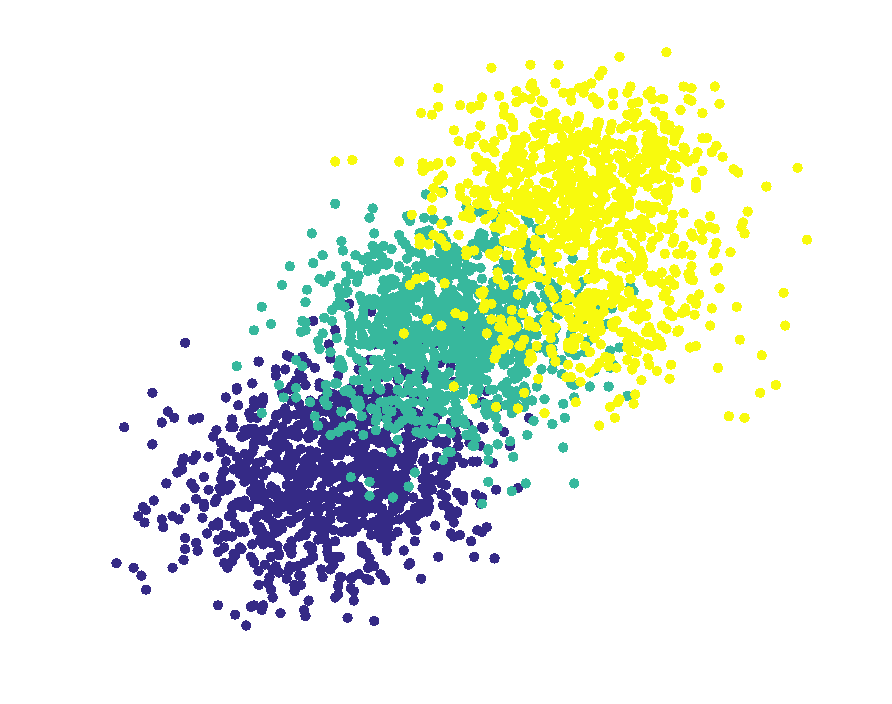
\includegraphics[width=\textwidth]{figures/scatter2}
\caption{The test dataset.}
\label{test}
\end{marginfigure}

The project is divided into four processing steps:
\begin{enumerate}
\item \textbf{generate}: generation of synthetic datasets
\item \textbf{train}: learning models
\item \textbf{probe}: probing models
\item \textbf{test}: predicting labels
\end{enumerate}

\subsection{\textbf{Generate step}: generation of the synthetic datasets}

The training and testing datasets are both of 3 classes each modeled as mixture of 3 Gaussians. 

\subsection{\textbf{Train step}: Learning models}

2 types of classifiers are considered. The nearest neighbors classifier is the simplest one. In this case, the classifier is entirely defined by the training data. Thus, no explicit modeling is performed. On contrary, the Gaussian mixture based approach needs to estimate a model for each class. In order to manipulate those models, the netlab\sidenote{\url{http://www.mathworks.com/matlabcentral/fileexchange/2654-netlab}} toolbox is used. This process is iterative and it can be interesting to see the impact of the number of iterations on the likelihood and also on the resulting classification accuracy.

Indeed, if increase and convergence of likelihood are mathematically ensured, the relation between the number of iterations and the accuracy is less straightforward. 

By default, explanes process the settings in unspecified order, especially in parallel mode. In order ot ensure the sequentiality of several settings related to a factor, one can set the said factor to be sequential:
\lstinputlisting[firstline=4, lastline=4]{../cldaFactors.txt}

At the first setting of the sequential run, explanes initializes \mcode{config.sequentialData} to an empty value. This variable can be used to store sequential data, in our case the GMM models.

The code for learning the GMMs thus reads:

\lstinputlisting[firstline=29, lastline=51]{../clda2train.m}

\subsection{\textbf{Probe step}: Probing models}

Once GMMs models are learned, one needs to compute their likelihood on some data, which can be done using the \mcode{gmmprobe} function:

\lstinputlisting[firstline=26, lastline=27]{../clda3probe.m}

\subsection{\textbf{Test step}: Predicting labels}

Predicting labels using the nearest neighbors approach is done using the \mcode{knn} and \mcode{knnfwd} functions:

\lstinputlisting[firstline=26, lastline=27]{../clda4test.m}

With the GMMs approach, one needs to collect the likelihoods of the GMMs each one modeling a given class and consider the GMM with the highest likelihood as the prediction:

\lstinputlisting[firstline=39, lastline=45]{../clda4test.m}

This explanes experiment is contracting, that is the number of settings for the third step is higher than the one for the fourth step, because the factor \mcode{class} is no longer needed at this last step. Thus the \mcode{data} structure is in this case an array with length equal to the number of classes which can be obtained by the following command:

\lstinputlisting[firstline=16, lastline=17]{../clda4test.m}

\section{Definition of factors}  


Those factors and their corresponding modalities are defined in the file named \texttt{cldaFactors.txt} whose content is the following:
\lstinputlisting{../cldaFactors.txt}

 Most the factor design discussed above is compactly displayed in Figure \ref{factorFlowGraph}.

\begin{figure}
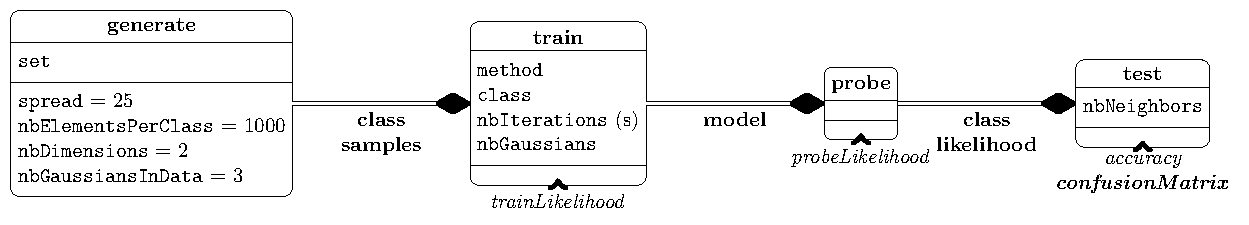
\includegraphics[width=\textwidth]{figures/factors}
\caption{Factor and data flow graph.}
\label{factorFlowGraph}
\end{figure}

\section{Results}






The analysis the performance of a classifier can be done using the confusion matrix. For this specific display, the observation is no longer an array but a structure that is filled as follow:

\lstinputlisting[firstline=55, lastline=59]{../clda4test.m}

On display, one needs to specify a given setting:

\lstinputlisting[firstline=16, lastline=16]{../cldaReport.m}

\begin{marginfigure}
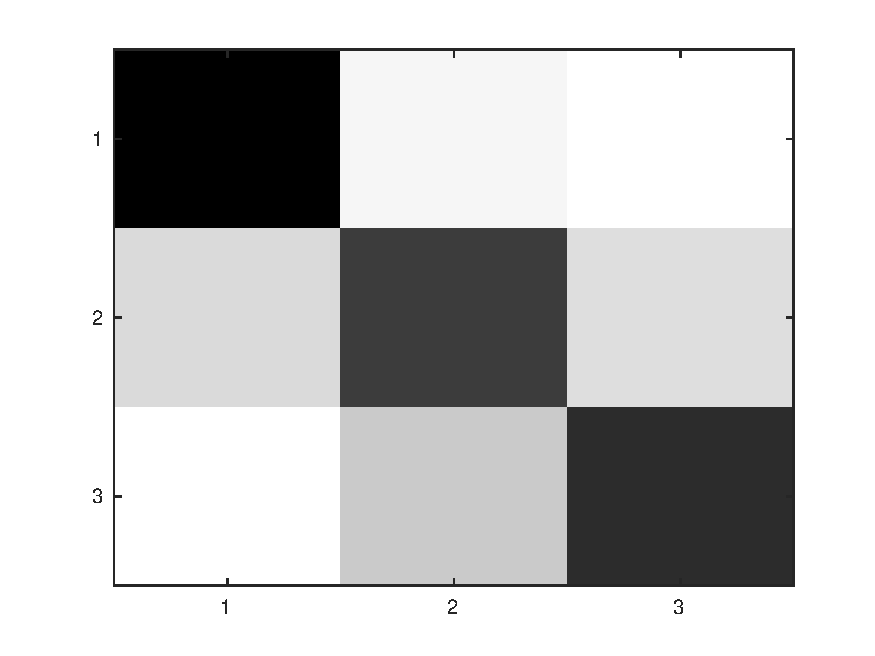
\includegraphics[width=\textwidth]{figures/confusion}
\caption{Confusion matrix for the method: gmm, set: test, nbIterations: 200, nbGaussians: 5.}
\label{confusion}
\end{marginfigure}

The resulting display shown on Figure \ref{confusion} is in line with the discrepancy of the training and testing dataset where the latter exhibit a stronger intrication between class 2 and 3, see Figures \ref{train} and \ref{test}.

\subsection{The KNN classifier}


\begin{marginfigure}
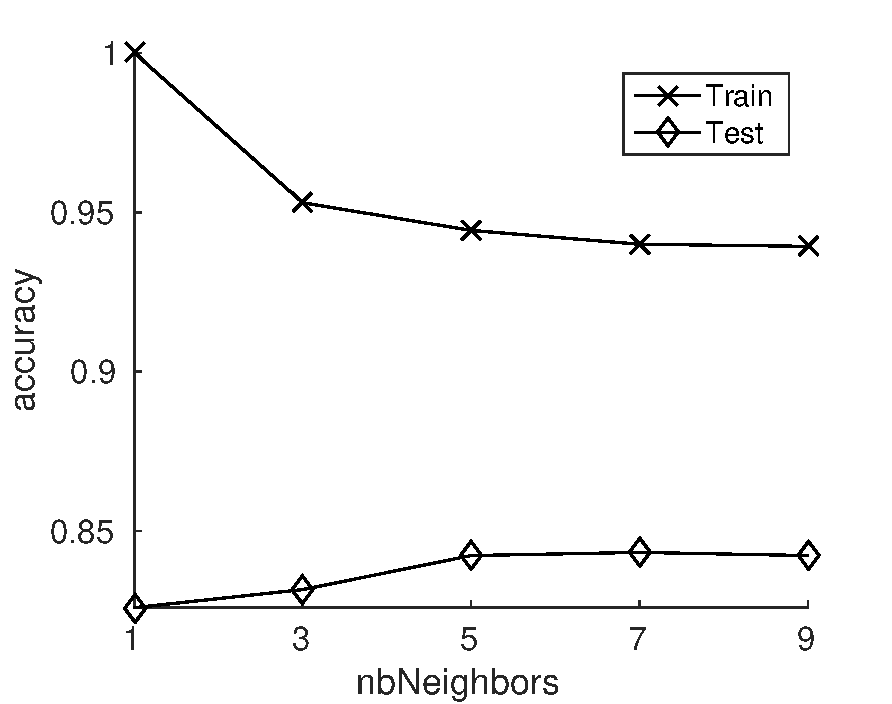
\includegraphics[width=\textwidth]{figures/knn}
\caption{Performance of the KNN classifier on the training and testing dataset.}
\label{knn}
\end{marginfigure}



The main parameter of this classifier is the number of neighbors. As can be seen on Figure \ref{knn}, the performance of the classifier on the testing dataset reaches a plateau around 5. As expected, the accuracy decreases with respect to the number of neighbors on the training dataset.

\subsection{The GMM classifier}

As can be seen on Figure \ref{like}, the quality of fit of each GMM increases with respect to the number of observations on the training dataset. On contrary, eventhough the difference is in this toy example negligible, the accuracy decreases with respect to the number of iterations, see Figure \ref{acc}. This is a common case with iterative methods suggesting a reduced number of iterations to avoid an overfit\marginnote{\url{https://en.wikipedia.org/wiki/Early_stopping}}.

\begin{marginfigure}
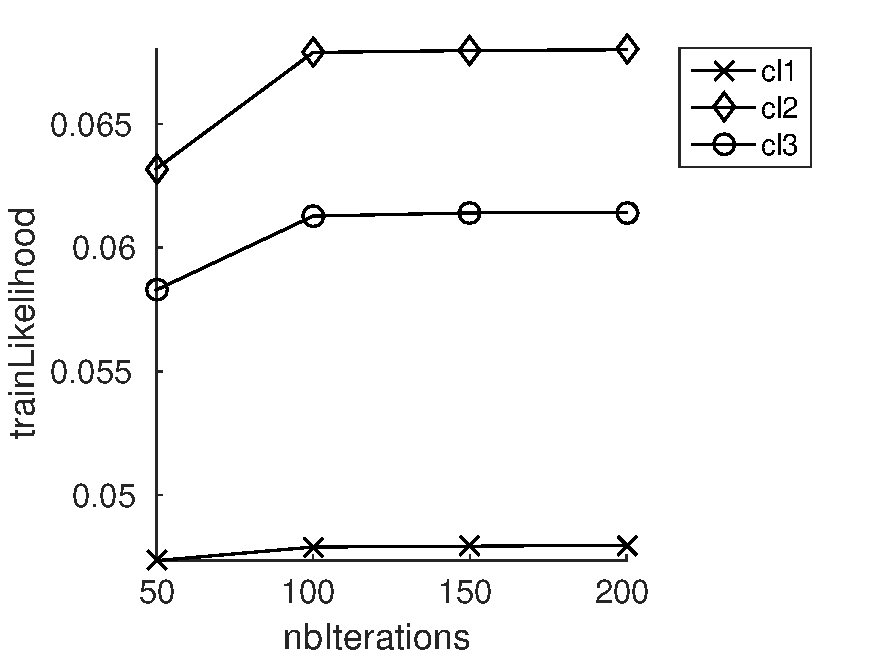
\includegraphics[width=\textwidth]{figures/likelihood}
\caption{Likelihood for the 3 GMMs models.}
\label{like}
\end{marginfigure}

\begin{marginfigure}
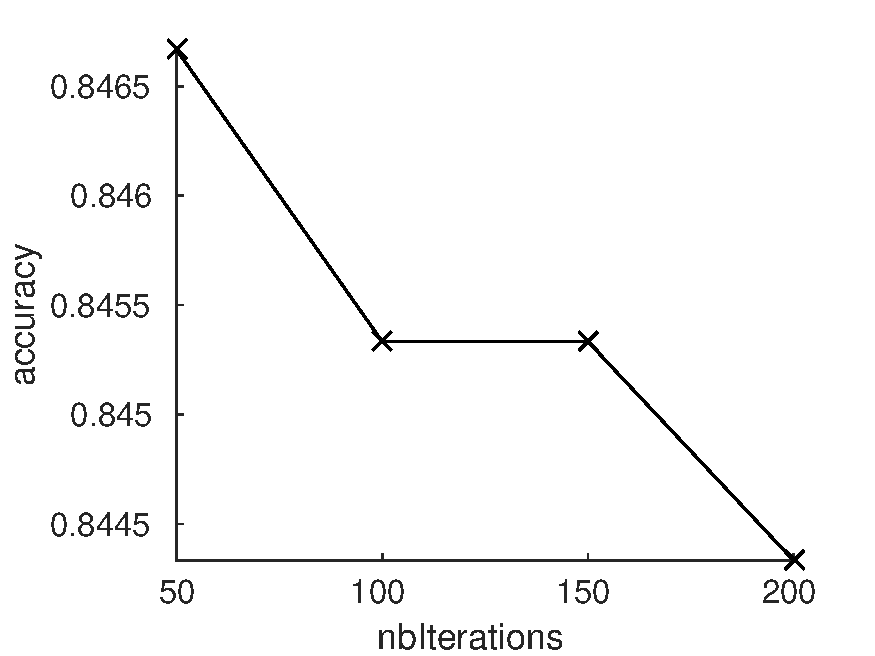
\includegraphics[width=\textwidth]{figures/accuracy}
\caption{Classification accuracy of the GMM clasifier.}
\label{acc}
\end{marginfigure}


\subsection{Overall}	

On this toy example, the GMM  and KKN classifiers achieves equivalent performances, see Figure \ref{overall}.

\begin{marginfigure}
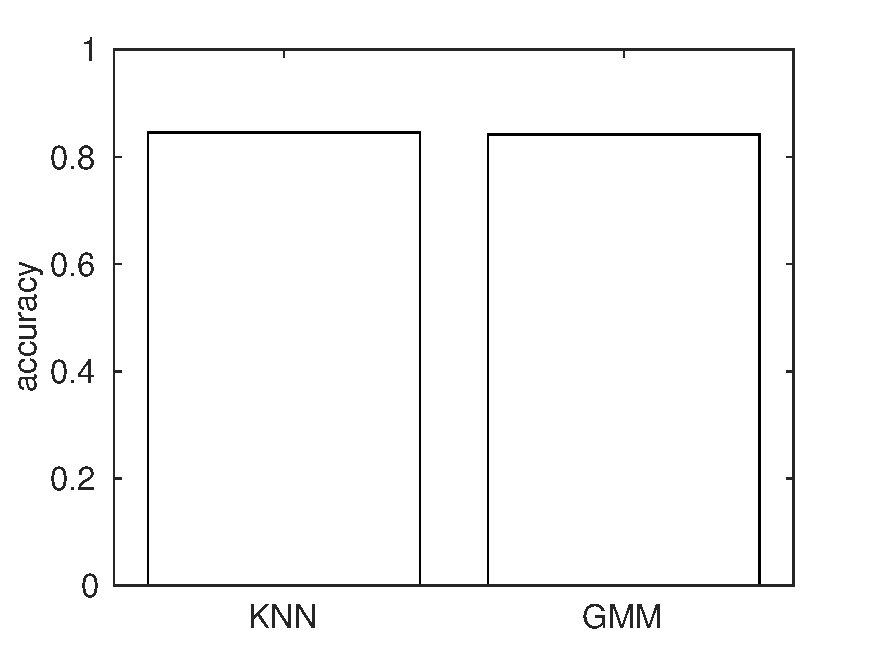
\includegraphics[width=\textwidth]{figures/overall}
\caption{Overall results.}
\label{overall}
\end{marginfigure}
  
%\input{tex/exposeTmp} % expLanesInsertionFlag DO NOT CLEAR (but move it where you want the generated temporary LaTEX code to be inserted) 
  
  
\bibliographystyle{abbrvnat} 
\bibliography{bib} 
  
\end{document} 
